% Options for packages loaded elsewhere
\PassOptionsToPackage{unicode}{hyperref}
\PassOptionsToPackage{hyphens}{url}
%
\documentclass[
  spanish,
]{book}
\usepackage{amsmath,amssymb}
\usepackage{lmodern}
\usepackage{iftex}
\ifPDFTeX
  \usepackage[T1]{fontenc}
  \usepackage[utf8]{inputenc}
  \usepackage{textcomp} % provide euro and other symbols
\else % if luatex or xetex
  \usepackage{unicode-math}
  \defaultfontfeatures{Scale=MatchLowercase}
  \defaultfontfeatures[\rmfamily]{Ligatures=TeX,Scale=1}
\fi
% Use upquote if available, for straight quotes in verbatim environments
\IfFileExists{upquote.sty}{\usepackage{upquote}}{}
\IfFileExists{microtype.sty}{% use microtype if available
  \usepackage[]{microtype}
  \UseMicrotypeSet[protrusion]{basicmath} % disable protrusion for tt fonts
}{}
\makeatletter
\@ifundefined{KOMAClassName}{% if non-KOMA class
  \IfFileExists{parskip.sty}{%
    \usepackage{parskip}
  }{% else
    \setlength{\parindent}{0pt}
    \setlength{\parskip}{6pt plus 2pt minus 1pt}}
}{% if KOMA class
  \KOMAoptions{parskip=half}}
\makeatother
\usepackage{xcolor}
\IfFileExists{xurl.sty}{\usepackage{xurl}}{} % add URL line breaks if available
\IfFileExists{bookmark.sty}{\usepackage{bookmark}}{\usepackage{hyperref}}
\hypersetup{
  pdftitle={Series de Tiempo},
  pdfauthor={Omar Rodríguez Torres (omarr667@ciencias.unam.mx)},
  pdflang={es},
  hidelinks,
  pdfcreator={LaTeX via pandoc}}
\urlstyle{same} % disable monospaced font for URLs
\usepackage{color}
\usepackage{fancyvrb}
\newcommand{\VerbBar}{|}
\newcommand{\VERB}{\Verb[commandchars=\\\{\}]}
\DefineVerbatimEnvironment{Highlighting}{Verbatim}{commandchars=\\\{\}}
% Add ',fontsize=\small' for more characters per line
\usepackage{framed}
\definecolor{shadecolor}{RGB}{248,248,248}
\newenvironment{Shaded}{\begin{snugshade}}{\end{snugshade}}
\newcommand{\AlertTok}[1]{\textcolor[rgb]{0.94,0.16,0.16}{#1}}
\newcommand{\AnnotationTok}[1]{\textcolor[rgb]{0.56,0.35,0.01}{\textbf{\textit{#1}}}}
\newcommand{\AttributeTok}[1]{\textcolor[rgb]{0.77,0.63,0.00}{#1}}
\newcommand{\BaseNTok}[1]{\textcolor[rgb]{0.00,0.00,0.81}{#1}}
\newcommand{\BuiltInTok}[1]{#1}
\newcommand{\CharTok}[1]{\textcolor[rgb]{0.31,0.60,0.02}{#1}}
\newcommand{\CommentTok}[1]{\textcolor[rgb]{0.56,0.35,0.01}{\textit{#1}}}
\newcommand{\CommentVarTok}[1]{\textcolor[rgb]{0.56,0.35,0.01}{\textbf{\textit{#1}}}}
\newcommand{\ConstantTok}[1]{\textcolor[rgb]{0.00,0.00,0.00}{#1}}
\newcommand{\ControlFlowTok}[1]{\textcolor[rgb]{0.13,0.29,0.53}{\textbf{#1}}}
\newcommand{\DataTypeTok}[1]{\textcolor[rgb]{0.13,0.29,0.53}{#1}}
\newcommand{\DecValTok}[1]{\textcolor[rgb]{0.00,0.00,0.81}{#1}}
\newcommand{\DocumentationTok}[1]{\textcolor[rgb]{0.56,0.35,0.01}{\textbf{\textit{#1}}}}
\newcommand{\ErrorTok}[1]{\textcolor[rgb]{0.64,0.00,0.00}{\textbf{#1}}}
\newcommand{\ExtensionTok}[1]{#1}
\newcommand{\FloatTok}[1]{\textcolor[rgb]{0.00,0.00,0.81}{#1}}
\newcommand{\FunctionTok}[1]{\textcolor[rgb]{0.00,0.00,0.00}{#1}}
\newcommand{\ImportTok}[1]{#1}
\newcommand{\InformationTok}[1]{\textcolor[rgb]{0.56,0.35,0.01}{\textbf{\textit{#1}}}}
\newcommand{\KeywordTok}[1]{\textcolor[rgb]{0.13,0.29,0.53}{\textbf{#1}}}
\newcommand{\NormalTok}[1]{#1}
\newcommand{\OperatorTok}[1]{\textcolor[rgb]{0.81,0.36,0.00}{\textbf{#1}}}
\newcommand{\OtherTok}[1]{\textcolor[rgb]{0.56,0.35,0.01}{#1}}
\newcommand{\PreprocessorTok}[1]{\textcolor[rgb]{0.56,0.35,0.01}{\textit{#1}}}
\newcommand{\RegionMarkerTok}[1]{#1}
\newcommand{\SpecialCharTok}[1]{\textcolor[rgb]{0.00,0.00,0.00}{#1}}
\newcommand{\SpecialStringTok}[1]{\textcolor[rgb]{0.31,0.60,0.02}{#1}}
\newcommand{\StringTok}[1]{\textcolor[rgb]{0.31,0.60,0.02}{#1}}
\newcommand{\VariableTok}[1]{\textcolor[rgb]{0.00,0.00,0.00}{#1}}
\newcommand{\VerbatimStringTok}[1]{\textcolor[rgb]{0.31,0.60,0.02}{#1}}
\newcommand{\WarningTok}[1]{\textcolor[rgb]{0.56,0.35,0.01}{\textbf{\textit{#1}}}}
\usepackage{longtable,booktabs,array}
\usepackage{calc} % for calculating minipage widths
% Correct order of tables after \paragraph or \subparagraph
\usepackage{etoolbox}
\makeatletter
\patchcmd\longtable{\par}{\if@noskipsec\mbox{}\fi\par}{}{}
\makeatother
% Allow footnotes in longtable head/foot
\IfFileExists{footnotehyper.sty}{\usepackage{footnotehyper}}{\usepackage{footnote}}
\makesavenoteenv{longtable}
\usepackage{graphicx}
\makeatletter
\def\maxwidth{\ifdim\Gin@nat@width>\linewidth\linewidth\else\Gin@nat@width\fi}
\def\maxheight{\ifdim\Gin@nat@height>\textheight\textheight\else\Gin@nat@height\fi}
\makeatother
% Scale images if necessary, so that they will not overflow the page
% margins by default, and it is still possible to overwrite the defaults
% using explicit options in \includegraphics[width, height, ...]{}
\setkeys{Gin}{width=\maxwidth,height=\maxheight,keepaspectratio}
% Set default figure placement to htbp
\makeatletter
\def\fps@figure{htbp}
\makeatother
\setlength{\emergencystretch}{3em} % prevent overfull lines
\providecommand{\tightlist}{%
  \setlength{\itemsep}{0pt}\setlength{\parskip}{0pt}}
\setcounter{secnumdepth}{5}
\usepackage{booktabs}
\usepackage{xcolor} 
\definecolor{gray97}{gray}{.97}
\definecolor{gray97}{gray}{.97}
\definecolor{airforceblue}{rgb}{0.36, 0.54, 0.66}
\definecolor{Mahogany}{rgb}{0.75, 0.25, 0.0}
\definecolor{Olive}{rgb}{0.5, 0.5, 0.0}
\definecolor{colortitulo}{RGB}{219,68,14} % 
\definecolor{colordominante}{RGB}{243,102,25}
\definecolor{colordominanteF}{RGB}{219,68,14}
\definecolor{colordominanteD}{RGB}{137,46,55}
\definecolor{mostaza}{RGB}{231,196,25}
\definecolor{amarilloM}{RGB}{248,199,90}
\definecolor{amarilloD}{RGB}{251,237,121}
\definecolor{grisamarillo}{RGB}{248,248,245} 
\definecolor{azulF}{rgb}{.0,.0,.3}
\definecolor{grisD}{rgb}{.3,.3,.3}
\definecolor{grisF}{rgb}{.82,.82,.82}
\definecolor{miverde}{RGB}{44,162,67}
\newcommand{\verde}{\color{miverde}}

\usepackage{listings}
% Puede usar lstlisting|texto| para código en el texto
\lstset{ 
	language=R,                     % the language of the code
	basicstyle=\footnotesize\ttfamily, % the size of the fonts that are used for the code
	%numbers=left,                   % where to put the line-numbers
	%numberstyle=\tiny\color{Blue},  % the style that is used for the line-numbers
	%stepnumber=1,                   % the step between two line-numbers. If it is 1, each line
	% will be numbered
	%numbersep=5pt,                  % how far the line-numbers are from the code
	frame=single,
	framextopmargin=3pt,
	framexbottommargin=3pt,
	framexleftmargin=0.4cm,
	backgroundcolor=\color{gray97},
	showspaces=false,               % show spaces adding particular underscores
	showstringspaces=false,         % underline spaces within strings
	showtabs=false,                 % show tabs within strings adding particular underscores
	frame=single,                   % adds a frame around the code
	rulecolor=\color{black},        % if not set, the frame-color may be changed on line-breaks within not-black text (e.g. commens (green here))
	tabsize=2,                      % sets default tabsize to 2 spaces
	captionpos=b,                   % sets the caption-position to bottom
	breaklines=true,                % sets automatic line breaking
	breakatwhitespace=false,        % sets if automatic breaks should only happen at whitespace
	keywordstyle=\color{Mahogany},      % keyword style
	commentstyle=\color{airforceblue},   % comment style
	stringstyle=\color{Olive}      % string literal style
} 


%\usepackage[width=17cm,height=23cm]{geometry}
%\geometry{bindingoffset=1.2cm}
\textheight=22cm
\textwidth=15.5cm
\topmargin=-1cm
\oddsidemargin = -0cm %margen izquierdo, página impar
\evensidemargin = -0cm %margen izquierdo, página par

\newcommand{\helv}{\fontfamily{phv}\fontsize{9}{11}\selectfont}


\usepackage{fancyhdr}
\pagestyle{fancy}

\renewcommand{\chaptermark}[1]{\markboth{#1}{}}
\renewcommand{\sectionmark}[1]{\markright{\thesection\ #1}}
\fancyhf{} % borra cabecera y pie actuales
\fancyhead[LE,RO]{\helv\thepage} %Left Even page - Right Odd page
\fancyhead[LO]{\helv\rightmark}
\fancyhead[RE]{\helv\leftmark}
%\renewcommand{\headrulewidth}{0pt} % Sin raya. Con raya?: cambiar {0} por {0.5pt}
%\renewcommand{\footrulewidth}{0pt}
\renewcommand{\headrulewidth}{0.5pt} % grosor 0.5pt
\addtolength{\headheight}{0.5pt} % espacio para la raya
\fancyheadoffset{0 cm} %Controla el tamaño de la línea



\usepackage{mdframed}

\usepackage{amsthm}
\newtheorem{theorem}{Teorema}[chapter]
\newtheorem{lemma}{Lema}[chapter]
\newtheorem{corollary}{Corolario}[chapter]
\newtheorem{proposition}{Proposición}[chapter]
\newtheorem{conjecture}{Conjecture}[chapter]

\newtheorem{del}{Definición}[chapter]
\newenvironment{definition}
{\begin{mdframed}[backgroundcolor=grisF, rightline=false,leftline=false,topline=false, bottomline=false]\begin{del}}
		{\end{del}\end{mdframed}}

\newtheorem{example}{Ejemplo}[chapter]
\newtheorem{exercise}{Ejercicio}[chapter]
\newtheorem{hypothesis}{Hypothesis}[chapter]
\theoremstyle{remark}
\newtheorem*{remark}{Nota: }
\newtheorem*{solution}{Solución}

\parskip=0.4cm
\parindent=3mm
\ifXeTeX
  % Load polyglossia as late as possible: uses bidi with RTL langages (e.g. Hebrew, Arabic)
  \usepackage{polyglossia}
  \setmainlanguage[]{spanish}
\else
  \usepackage[main=spanish]{babel}
% get rid of language-specific shorthands (see #6817):
\let\LanguageShortHands\languageshorthands
\def\languageshorthands#1{}
\fi
\ifLuaTeX
  \usepackage{selnolig}  % disable illegal ligatures
\fi
\usepackage[]{natbib}
\bibliographystyle{apalike}

\title{Series de Tiempo}
\author{Omar Rodríguez Torres (\href{mailto:omarr667@ciencias.unam.mx}{\nolinkurl{omarr667@ciencias.unam.mx}})}
\date{2021-07-07}

\begin{document}
\maketitle

{
\setcounter{tocdepth}{1}
\tableofcontents
}
\hypertarget{pruxf3logo}{%
\chapter*{Prólogo}\label{pruxf3logo}}
\addcontentsline{toc}{chapter}{Prólogo}

Estas notas corresponden al curso de Modelos de Supervivencia y de Series de Tiempo contemplados en el \href{http://www.fciencias.unam.mx/licenciatura/asignaturas/2017/1739}{plan de estudio} en la Facultad de Ciencias de la Universidad Nacional Autónoma de México para las licenciaturas de actuaría, matemáticas y matemáticas aplicadas.

El siguiente texto esta enfocado para los interesados que desean abordar el tema de series de tiempo, aunque su lectura puede ser relevante para cualquier interesado se desea que el lector tenga conocimientos solidos en probabilidad y en temas de estadística inferencial, así por la naturaleza de este curso, se tenga noción de las funciones básicas de programación en R.

Este texto fue generado en bookdown a través de R 3.6.3, con el entorno de desarrollo (IDE) Rstudio, así como el texto PDF generado a por medio de LATEX. Para generar el libro (compilar) puede ser recomendable instalar la última versión de \href{(https://www.rstudio.com/products/rstudio/download/)}{RStudio} y la versión de desarrollo de \texttt{bookdown} disponible en \href{https://github.com/rstudio/bookdown}{Github}.

\begin{flushleft}
\includegraphics[width=1.22in]{images/by-sa-88x31} \end{flushleft}

Esta obra está bajo una licencia de \href{https://creativecommons.org/licenses/by-sa/4.0/deed.es}{Creative Commons Reconocimiento-CompartirIgual 4.0 Internacional}.

\hypertarget{series-de-tiempo}{%
\chapter{Series de Tiempo}\label{series-de-tiempo}}

\hypertarget{introducciuxf3n}{%
\section{Introducción}\label{introducciuxf3n}}

El ser humano desde que es consciente del tiempo se encuentra interesado en predecir eventos futuros y con ello estar preparados para afrontar dichos sucesos; de esta forma los primeros humanos podrían haberse interesados en eventos ambientales como ¿El día de mañana habrá un buen clima? ¿Encontraremos alimento y agua suficiente? etcétera. Las personas con más experiencia, con conocimiento más empírico, podrían tener una noción del clima viendo el cielo, nubes o inclusive las constelaciones para detectar en la temporada en la que se encontraban y así hacer un pronóstico.

En tiempos posteriores, saciando los requerimientos básicos de vida (alimento, vestido, vivienda), los aspectos que querían conocer del futuro eran otros, por lo que, viendo la inquietud incesante de los seres humanos sobre el tema, surgen aspectos místicos, mitológicos e inclusive mágicos, que buscan dar respuestas a estas inquietudes. Así es como surgen en todas las partes del mundo profecías, desde los mexicas en el que tenía profetizado la llegada de Quetzalcóatl o establecimiento de la ciudad de Tenochtitlan, en Grecia con los oráculos, el cual es una respuesta dada por un dios a una pregunta personal, concerniente generalmente al futuro, como método de adivinación, el cual posiblemente el oráculo más famoso puede consultarse en la tragedia griega de Edipo Rey, o las profecías establecidas en la biblia. Aunque muchos de estos elementos han desaparecidos, existen otros que están muy presentes en nuestra cultura, principalmente en la religión, pero también ha cobrado relevancia los chamanes, adivinos, profetas, lectura de tarot, hasta las galletas chinas de la suerte tienen como finalidad predecir el futuro inmediato, de manera subsecuente, brinda a las personas a una situación de tranquilidad o preparación sobre el pronóstico dado.

Todos estos pronósticos son basados en conocimiento empírico de los practicantes, sin cuestionar la efectividad de las predicciones, muchas de ellas no son métodos demasiados exactos o carecen de rigurosidad pues son temas un tanto subjetivos a los ojos del practicante, por ejemplo, en la lectura de cartas cada tarotista puede tener un concepto o idea diferente en la interpretación de cada carta; además la experiencia, aunque es buena, muchas veces puede fallar, por ejemplo puede haber días nublados en el que muchos pensarían que va a llover, sin embargo, termina el día sin que caiga alguna gota del cielo, otro ejemplo sería pronosticar el clima en verano, aunque la mayoría de las veces los días son calurosos en esta época, no se podría afirmar que todos los días sean cálidos pues puede existir algún día en el que el clima sea frío aún en verano, es por eso que es de gran importancia crear métodos estadísticos que contengan un mayor rigor matemático, sean reproducible para cualquier persona y sean más objetivos en su análisis.

Desde el lado científico, por medio de modelos estadísticos y matemáticos, también se ha buscado dar solución a la inquietud sobre el futuro, por lo que se han desarrollado diversos modelos que buscan proyectar la información y así poder tener un bosquejo de los datos en tiempos posteriores para que así se disminuya la incertidumbre del futuro y tanto personas, empresas y gobiernos puedan definir una estrategia y planeación hacia ese futuro estimado.

Desde luego cada modelo tiene una serie de requerimientos y objetivos diferentes, pero de manera general todos los modelos requieren que los datos a estimar sean cuantificables de una manera estándar para todas las observaciones, para ello usan información del pasado y presente para así proyectar la información a un tiempo posterior del que se tiene registro. Además dichos modelos buscan disminuir el error en la estimación, es decir, cada modelo busca que la diferencia entre la observación real y la esperada sean lo más similar posible.

Uno de esos modelos es el análisis de series de tiempo, en dicho modelo se busca encontrar tendencias entenderlas y así proyectar los datos con técnicas que se estarán abordando más adelante, para dicho estudio se requerirá una serie de datos a lo largo del tiempo, para ello se definirá a una serie de tiempo como:

\begin{definition}
\protect\hypertarget{def:unlabeled-div-1}{}\label{def:unlabeled-div-1}

Una serie de tiempo es una secuencia ordenada cronológicamente de observaciones cuantitativas que se encuentran espaciadas entre sí de manera uniforme.

\end{definition}

En las series de tiempo se analiza las observaciones en el pasado para así predecir el futuro, lo que permite gestionar y tomar decisiones con la debida información. Un análisis de series de tiempo cuantifica las principales características de los datos y las variaciones aleatorias. Por estas razones, combinadas con la mejora de los sistemas computacionales, han hecho que los métodos de series temporales se apliquen ampliamente en la administración, la industria y el comercio.

Una serie de tiempo se dice que es \textbf{continua} cuando sus observaciones ocurren en un tiempo continuo, por ejemplo, el mercado accionario tiene este tipo de comportamiento pues en cada instante dentro del horario bancario existe un precio nuevo como respuesta a los flujos de mercado en ese momento, cabe destacar que una serie puede ser continua, aunque el valor de la variable de interés se comporte de manera discreta. De manera análoga, una serie puede considerarse discreta cuando las observaciones ocurren de una manera discreta, es decir, las observaciones son registradas de manera espaciada y uniforme entre sí a o lo largo del tiempo.

Este texto se enfocará principalmente a la serie de tiempo discreta, por lo que a menos que se especifique lo contrario, al referirse a una serie de tiempo se supondrá que los tiempos ocurren de manera espaciada entre sí. Cabe mencionar que en caso de existir una serie de tiempo continua se podrá transformar en una serie de tiempo discreta, tomando medidas resumen en un periodo de tiempo discreto, por ejemplo, en el mercado accionario, aunque el precio sea continuo, al final del día se muestra el precio final con el que cerro la acción, otras medidas puede ser la suma o promedio de todas las precipitaciones captada durante un mes.

En la industria, comercio, ciencia, así como en la mayoría de las ramas académicas y profesionales se miden variables cuantitativas de manera secuencial en el tiempo. Por ejemplo, en economía, las \textbf{tasas de interés y las tasas de cambio} se registran cada día, basta consultar algún sitio web financiero para obtener el valor de las tasas a lo largo del tiempo, por la naturaleza del mismo, se tiene una periodicidad de información diaria (en acciones y algunos instrumentos financieros, la periodicidad es diaria omitiendo fines de semana y días festivos), sin embargo, dependiendo de la variable de interés se pueden seleccionar intervalos de tiempo diferentes, por ejemplo: la cantidad de \textbf{lluvia} registrada en un pluviómetro en una cierta zona se puede registrar de manera mensual representando el promedio de mm de agua caída; los cambios de \textbf{temperaturas} a lo largo del día se pueden medir cada hora en una estación meteorológica; o por ejemplo el \textbf{Producto Interno Bruto (PIB) } de un cierto país calculado trimestralmente. De manera general, cuando una variable cuantitativa se mide secuencialmente en el tiempo durante un intervalo fijo (o intervalo de muestreo), los datos forman una serie de tiempo.

A lo largo de este texto se representará a la serie de tiempo de tamaño \(n\) con la notación: \[\left\{x_t : t=1,\ldots, n\right\},\] por lo que cada observación de la serie es representada como
\[\left\{x_1,x_2, \ldots, x_n\right\}.\]

Para fines convivencia, se supondrá que la abreviación \(x_t\) hace referencia a una serie de tiempo en el \(t\)-ésimo momento de tamaño \(n\), a menos de que se especifique lo contrario, donde \(0< t \le n\). Mientras que la abreviación \(\hat{x}_t\) hace referencia al valor estimado por el modelo de serie de tiempo elegido.

Algunos libros hacen notar que:

\begin{itemize}
\item
  Si \(t\le n\) entonces se le conocen a \(\hat{x}_t\) como predicción (prediction)
\item
  Si \(t > n\) entonces se le conocen a \(\hat{x}_t\) como pronóstico (forecast)
\end{itemize}

A diferencia de mucha de la teoría estadística, la cual se basa en muestras aleatorias de observaciones independientes, en series de tiempo se establece que las observaciones dependen de cierta medida una de la otra, es de gran importancia resaltar esta idea ya que si las observaciones dependen en gran medida de otras observaciones entonces se puede encontrar esta relación y así poder estimar valores futuros a partir de valores ya conocidos. Si los datos fueran independientes entre sí, se tendría un comportamiento prácticamente aleatorio por lo que no se podría realizar buenas predicciones. Si la serie de tiempo puede ser predicha exactamente por un modelo de series de tiempo, entonces se dice que la serie es \textbf{determinista}, de lo contrario se dice que la serie es \textbf{estocástica}, sin embargo, un buen modelo, aunque no sea determinista, puede ayudar a identificar situaciones que se podrían presentar en un futuro inmediato calculado a partir de las observaciones con las que se tiene registro.

\hypertarget{objetivos-del-anuxe1lisis-de-series-de-tiempo}{%
\section{Objetivos del análisis de series de tiempo}\label{objetivos-del-anuxe1lisis-de-series-de-tiempo}}

Como anteriormente de manera general se describió la elaboración de un análisis de series de tiempo es muy útil ya que proporciona varios elementos que pueden ser analizados para describir, comprender, explicar, estimar y prevenir el suceso o fenómeno que se estudia:

\hypertarget{describir}{%
\subsubsection*{Describir}\label{describir}}
\addcontentsline{toc}{subsubsection}{Describir}

Generalmente en un análisis de series de tiempo, el primer paso es graficar la información, ya que visualmente se pueden detectar muchas de las características de la información analizada, por ejemplo, se puede detectar la tendencia de la serie, identificar patrones que los datos van siguiendo a lo largo del tiempo, identificar unidades de tendencia central como la media, moda, rango, así como identificar mínimos, máximo, valores atípicos, y variación de la información, más adelante se hablará con más detalle de algunas de estas propiedades.\\
De igual menara describir estos elementos nos ayuda a describir si un análisis de series de tiempo puede ser o no elaborado. Por ejemplo, si la serie tiene un comportamiento completamente aleatorio tendríamos que optar por otros métodos. De igual forma si la serie tiene valores atípicos tendríamos que dar solución a esas observaciones. El tratamiento de valores atípicos es un tema bastante complejo en el que se tiene que respaldar con teoría y con práctica, ya que si consideramos este valor extremo puede que el punto de influencia se alto y el resultado sea alterado por este valor, si lo quitamos entonces podríamos sobreajustar el modelo y nuevamente el resultado no sería adecuado. Para estos casos en particular se debe ajustar modelos robustos ya que no son sensibles a valores atípicos.

\hypertarget{explicaciuxf3n}{%
\subsubsection*{Explicación}\label{explicaciuxf3n}}
\addcontentsline{toc}{subsubsection}{Explicación}

En la siguiente sección se analizará series de tiempo más específicas, sin embargo, en muchas series la información tiene aspectos de gran relevancia tal como la tendencia y periodicidad, por ejemplo, si se consulta el PIB de los Estados Unidos de 1960 a 2019, el lector puede observar que el valor del PIB tiene una tendencia positiva ya que ha estado en un gran crecimiento prácticamente exponencial, es decir, año con año el PIB aumenta mostrando que existe una tendencia positiva de los datos. Pero no sólo la tendencia puede ser apreciada, también en muchas otras series puede observarse que existe información que sigue un patrón año con año, por ejemplo, supongamos un país cualquiera, si analizara el PIB posiblemente en la temporada de invierno, cuarto trimestre del año, el PIB podría aumentar considerablemente por el gran derrame económico que implica vacaciones y época decembrina, sin embargo, un trimestre posterior también puede observarse que debido al gasto ocasionado en el cuarto trimestre, el PIB puede disminuir pues la demanda de servicios y productos es menor, este ciclo puede observarse que se repite año tras año y esto es a lo que en un primer momento denominaremos \textbf{periodicidad} o \textbf{variación estacional}

\hypertarget{predicciuxf3n}{%
\subsubsection*{Predicción}\label{predicciuxf3n}}
\addcontentsline{toc}{subsubsection}{Predicción}

Dada una secuencia de series de tiempo, después de entender y dar explicación al comportamiento de los datos, el lector puede estar interesado en hacer pronostico o predicciones con las técnicas que estemos analizado a lo largo de este texto

\hypertarget{control}{%
\subsubsection*{Control}\label{control}}
\addcontentsline{toc}{subsubsection}{Control}

Una vez hecha una predicción, las estimaciones deben pasar por un proceso de evaluación; como primera medida, debemos de graficar las observaciones reales con las observaciones estimadas para ver si visualmente tiene un comportamiento deseado. Hay técnicas más avanzadas como \emph{cross-validation} o validación cruzada en la que se forman dos bases de datos una base de entrenamiento en el que cual se trabaja y se construyen los modelos y una de pruebas donde se observa si el modelo puede ser replicado y da los resultados esperados. Más adelante se detallará este proceso de control y de aceptación del modelo

\hypertarget{ejemplo-de-series-de-tiempo}{%
\section{Ejemplo de series de tiempo}\label{ejemplo-de-series-de-tiempo}}

A lo largo de este texto se trabajará con diversas bases de datos, las cuales se estará definiendo en cada ejercicio que se realice, sin embargo, la teoría a desarrollar se basará en 3 diferentes series de tiempo, las cuales se mencionarán a continuación:

\hypertarget{consumo-de-energuxeda-eluxe9ctrica-domuxe9stica}{%
\subsection{Consumo de energía eléctrica doméstica}\label{consumo-de-energuxeda-eluxe9ctrica-domuxe9stica}}

El Instituto Nacional de Estadística y Geografía (INEGI) publica de manera mensual una serie de valores económicos de México, uno de ellos hace referencia al consumo de energía eléctrica doméstica total en miles de millones de watts/hora en el territorio mexicano, por practicidad a esta serie de tiempo se le denominará CONELDO.

Para este trabajó se extrajo de manera mensual, desde la página oficial del INEGI, el consumo de energía eléctrica acumulado en el periodo desde enero 2009 hasta diciembre 2017, dichos resultados serán mostrados por medio del siguiente vector, recuerde que un vector en R, debe iniciar por la letra c, prefijo de concatenate, seguido de paréntesis y dentro de ellos se ingresa cada observación separado por comas.

\begin{Shaded}
\begin{Highlighting}[]
\NormalTok{CONELDO}\OtherTok{=}\FunctionTok{c}\NormalTok{(}\DecValTok{2861}\NormalTok{, }\DecValTok{2833}\NormalTok{,   }\DecValTok{2686}\NormalTok{,   }\DecValTok{2798}\NormalTok{,   }\DecValTok{3123}\NormalTok{,   }\DecValTok{3232}\NormalTok{,   }\DecValTok{3377}\NormalTok{,   }\DecValTok{3545}\NormalTok{,   }\DecValTok{3558}\NormalTok{,   }
          \DecValTok{3275}\NormalTok{, }\DecValTok{3079}\NormalTok{,   }\DecValTok{2792}\NormalTok{,   }\DecValTok{2825}\NormalTok{,   }\DecValTok{2769}\NormalTok{,   }\DecValTok{2655}\NormalTok{,   }\DecValTok{2735}\NormalTok{,   }\DecValTok{2996}\NormalTok{,   }\DecValTok{3282}\NormalTok{,}
          \DecValTok{3594}\NormalTok{, }\DecValTok{3544}\NormalTok{,   }\DecValTok{3633}\NormalTok{,   }\DecValTok{3422}\NormalTok{,   }\DecValTok{3220}\NormalTok{,   }\DecValTok{2859}\NormalTok{,   }\DecValTok{2998}\NormalTok{,   }\DecValTok{3062}\NormalTok{,   }\DecValTok{2907}\NormalTok{,}
          \DecValTok{3012}\NormalTok{, }\DecValTok{3349}\NormalTok{,   }\DecValTok{3537}\NormalTok{,   }\DecValTok{3688}\NormalTok{,   }\DecValTok{3632}\NormalTok{,   }\DecValTok{3792}\NormalTok{,   }\DecValTok{3608}\NormalTok{, }\DecValTok{3274}\NormalTok{, }\DecValTok{3049}\NormalTok{,}
          \DecValTok{2999}\NormalTok{, }\DecValTok{2990}\NormalTok{,   }\DecValTok{2983}\NormalTok{,   }\DecValTok{3068}\NormalTok{,   }\DecValTok{3279}\NormalTok{,   }\DecValTok{3440}\NormalTok{,   }\DecValTok{3636}\NormalTok{,   }\DecValTok{3670}\NormalTok{,   }\DecValTok{3835}\NormalTok{,}
          \DecValTok{3605}\NormalTok{, }\DecValTok{3436}\NormalTok{,   }\DecValTok{3126}\NormalTok{,   }\DecValTok{3126}\NormalTok{,   }\DecValTok{3120}\NormalTok{,   }\DecValTok{2905}\NormalTok{,   }\DecValTok{2992}\NormalTok{,   }\DecValTok{3272}\NormalTok{,   }\DecValTok{3524}\NormalTok{,}
          \DecValTok{3732}\NormalTok{, }\DecValTok{3807}\NormalTok{,   }\DecValTok{3793}\NormalTok{,   }\DecValTok{3631}\NormalTok{,   }\DecValTok{3481}\NormalTok{,   }\DecValTok{3203}\NormalTok{,   }\DecValTok{3230}\NormalTok{,   }\DecValTok{3176}\NormalTok{,   }\DecValTok{3005}\NormalTok{,   }
          \DecValTok{3119}\NormalTok{, }\DecValTok{3382}\NormalTok{,   }\DecValTok{3543}\NormalTok{,   }\DecValTok{3820}\NormalTok{,   }\DecValTok{3985}\NormalTok{,   }\DecValTok{3950}\NormalTok{,   }\DecValTok{3743}\NormalTok{,   }\DecValTok{3512}\NormalTok{,   }\DecValTok{3211}\NormalTok{,}
          \DecValTok{3229}\NormalTok{, }\DecValTok{3212}\NormalTok{,   }\DecValTok{3043}\NormalTok{,   }\DecValTok{3188}\NormalTok{,   }\DecValTok{3483}\NormalTok{,   }\DecValTok{3678}\NormalTok{,   }\DecValTok{3896}\NormalTok{,   }\DecValTok{4142}\NormalTok{,   }\DecValTok{4190}\NormalTok{,   }
          \DecValTok{4063}\NormalTok{, }\DecValTok{3847}\NormalTok{,   }\DecValTok{3482}\NormalTok{,   }\DecValTok{3415}\NormalTok{,   }\DecValTok{3330}\NormalTok{,   }\DecValTok{3063}\NormalTok{,   }\DecValTok{3284}\NormalTok{, }\DecValTok{3677}\NormalTok{, }\DecValTok{3964}\NormalTok{,}
          \DecValTok{4211}\NormalTok{, }\DecValTok{4296}\NormalTok{,   }\DecValTok{4310}\NormalTok{,   }\DecValTok{4142}\NormalTok{,   }\DecValTok{3858}\NormalTok{,   }\DecValTok{3591}\NormalTok{,   }\DecValTok{3371}\NormalTok{,   }\DecValTok{3331}\NormalTok{,   }\DecValTok{3297}\NormalTok{,}
          \DecValTok{3396}\NormalTok{, }\DecValTok{3753}\NormalTok{,   }\DecValTok{3967}\NormalTok{,   }\DecValTok{4322}\NormalTok{,   }\DecValTok{4341}\NormalTok{,   }\DecValTok{4398}\NormalTok{,   }\DecValTok{4213}\NormalTok{,   }\DecValTok{3867}\NormalTok{,   }\DecValTok{3509}\NormalTok{)}

\FunctionTok{print}\NormalTok{(CONELDO)}
\end{Highlighting}
\end{Shaded}

\begin{verbatim}
##   [1] 2861 2833 2686 2798 3123 3232 3377 3545 3558 3275 3079 2792 2825 2769 2655
##  [16] 2735 2996 3282 3594 3544 3633 3422 3220 2859 2998 3062 2907 3012 3349 3537
##  [31] 3688 3632 3792 3608 3274 3049 2999 2990 2983 3068 3279 3440 3636 3670 3835
##  [46] 3605 3436 3126 3126 3120 2905 2992 3272 3524 3732 3807 3793 3631 3481 3203
##  [61] 3230 3176 3005 3119 3382 3543 3820 3985 3950 3743 3512 3211 3229 3212 3043
##  [76] 3188 3483 3678 3896 4142 4190 4063 3847 3482 3415 3330 3063 3284 3677 3964
##  [91] 4211 4296 4310 4142 3858 3591 3371 3331 3297 3396 3753 3967 4322 4341 4398
## [106] 4213 3867 3509
\end{verbatim}

El vector que se acaba de construir recibe el nombre de CONELDO, la anterior ejecución provocó que los valores se cargaran en el espacio de trabajo dentro de la memoria del equipo donde se ejecutó, sin embargo, aún el tiempo no se encuentra indexado, para ello necesitamos construir un objeto de series de tiempo dentro de R, la declaración de este objeto es de la forma:

\begin{verbatim}
ts(vector, start=c(anio, periodo), frequency=frecuencia)
\end{verbatim}

Donde \emph{start}, es un vector con el año y el periodo del primer dato y \emph{frequency} la frecuencia en el que se registran los datos. Siguiendo la anterior descripción podemos convertir el vector CONELDO en un objeto de series de tiempo que denominaremos CONELDO.ts

\begin{Shaded}
\begin{Highlighting}[]
\CommentTok{\#Se convierte la base en un modelo de series de tiempo}
\NormalTok{CONELDO.ts}\OtherTok{=}\FunctionTok{ts}\NormalTok{(CONELDO,}\AttributeTok{start =}\DecValTok{2009}\NormalTok{,}\AttributeTok{frequency =} \DecValTok{12}\NormalTok{)}
\FunctionTok{print}\NormalTok{(CONELDO.ts)}
\end{Highlighting}
\end{Shaded}

\begin{verbatim}
##       Jan  Feb  Mar  Apr  May  Jun  Jul  Aug  Sep  Oct  Nov  Dec
## 2009 2861 2833 2686 2798 3123 3232 3377 3545 3558 3275 3079 2792
## 2010 2825 2769 2655 2735 2996 3282 3594 3544 3633 3422 3220 2859
## 2011 2998 3062 2907 3012 3349 3537 3688 3632 3792 3608 3274 3049
## 2012 2999 2990 2983 3068 3279 3440 3636 3670 3835 3605 3436 3126
## 2013 3126 3120 2905 2992 3272 3524 3732 3807 3793 3631 3481 3203
## 2014 3230 3176 3005 3119 3382 3543 3820 3985 3950 3743 3512 3211
## 2015 3229 3212 3043 3188 3483 3678 3896 4142 4190 4063 3847 3482
## 2016 3415 3330 3063 3284 3677 3964 4211 4296 4310 4142 3858 3591
## 2017 3371 3331 3297 3396 3753 3967 4322 4341 4398 4213 3867 3509
\end{verbatim}

Nótese que como la información empieza en el primer periodo del año 2009 se puede abreviar el parámetro start sólo como 2009, además observe que en este último bloque de código el tiempo se encuentra indexado. Ya que se indicó una periodicidad igual a 12, R entiende que se está ingresando datos de manera mensual por lo que lo acomodará el resultado en un arreglo donde cada columna corresponde a un mes y cada renglón a un año. Al tener indexado el tiempo se puede apreciar que se tiene acceso a funciones de identificación como, \emph{class()} para identificar la clase del objeto que se acaba de crear, \emph{start()} para identificar el comienzo de los datos, \emph{end()} para encontrar el tiempo de la última observación, \emph{frequency()} para mostrar la frecuencia de la serie, \emph{summary()} para obtener algunas de las medidas básicas como media, mediana, cuartiles, mínimos y máximos, \emph{cycle()} para mostrar el ciclo que sigue los datos en el tiempo dependiendo de la frecuencia dada.

\begin{Shaded}
\begin{Highlighting}[]
\FunctionTok{class}\NormalTok{(CONELDO.ts)}\CommentTok{\#El formato de la serie de tiempo es}
\end{Highlighting}
\end{Shaded}

\begin{verbatim}
## [1] "ts"
\end{verbatim}

\begin{Shaded}
\begin{Highlighting}[]
\FunctionTok{start}\NormalTok{(CONELDO.ts)}\CommentTok{\#El incio de la serie de tiempo es}
\end{Highlighting}
\end{Shaded}

\begin{verbatim}
## [1] 2009    1
\end{verbatim}

\begin{Shaded}
\begin{Highlighting}[]
\FunctionTok{frequency}\NormalTok{(CONELDO.ts)}\CommentTok{\#La frecuencia de la serie de tiempo es}
\end{Highlighting}
\end{Shaded}

\begin{verbatim}
## [1] 12
\end{verbatim}

\begin{Shaded}
\begin{Highlighting}[]
\FunctionTok{summary}\NormalTok{(CONELDO.ts) }\CommentTok{\#Información de la distribución de los datos}
\end{Highlighting}
\end{Shaded}

\begin{verbatim}
##    Min. 1st Qu.  Median    Mean 3rd Qu.    Max. 
##    2655    3120    3406    3438    3699    4398
\end{verbatim}

\begin{Shaded}
\begin{Highlighting}[]
\FunctionTok{cycle}\NormalTok{(CONELDO.ts)  }\CommentTok{\#Ciclos de la serie de tiempo}
\end{Highlighting}
\end{Shaded}

\begin{verbatim}
##      Jan Feb Mar Apr May Jun Jul Aug Sep Oct Nov Dec
## 2009   1   2   3   4   5   6   7   8   9  10  11  12
## 2010   1   2   3   4   5   6   7   8   9  10  11  12
## 2011   1   2   3   4   5   6   7   8   9  10  11  12
## 2012   1   2   3   4   5   6   7   8   9  10  11  12
## 2013   1   2   3   4   5   6   7   8   9  10  11  12
## 2014   1   2   3   4   5   6   7   8   9  10  11  12
## 2015   1   2   3   4   5   6   7   8   9  10  11  12
## 2016   1   2   3   4   5   6   7   8   9  10  11  12
## 2017   1   2   3   4   5   6   7   8   9  10  11  12
\end{verbatim}

La ventaja de convertir datos en objetos de serie de tiempo es que facilita el trabajo y análisis de muchos de estos modelos pues al indexar en una misma variable, el valor de cada observación, así como el tiempo de ocurrencia, evita la sobrecarga de memoria y declaración de variables. Por ejemplo, siguiendo la idea básica de programación en R, se tendría que manejar una variable de tiempo y otra de datos, así para poder graficar una serie de tiempo podría realizarse el siguiente código:

\begin{Shaded}
\begin{Highlighting}[]
\FunctionTok{library}\NormalTok{(ggplot2) }\CommentTok{\#Librería a ocupar para graficar}

\DocumentationTok{\#\# Se crea una tabla en la cual se tenga los datos y las fechas}
\NormalTok{CONELDO.base }\OtherTok{=} \FunctionTok{data.frame}\NormalTok{(CONELDO, }
                          \AttributeTok{time =} \FunctionTok{seq}\NormalTok{(}\FunctionTok{ISOdate}\NormalTok{(}\DecValTok{2009}\NormalTok{,}\DecValTok{01}\NormalTok{,}\DecValTok{01}\NormalTok{), }
                                     \FunctionTok{ISOdate}\NormalTok{(}\DecValTok{2017}\NormalTok{,}\DecValTok{12}\NormalTok{,}\DecValTok{01}\NormalTok{),}
                                     \AttributeTok{by =} \StringTok{"month"}\NormalTok{) }
\NormalTok{                          )}
\DocumentationTok{\#\# Se imprime en pantalla los primeros 5 renglones}
\FunctionTok{head}\NormalTok{(CONELDO.base)}
\end{Highlighting}
\end{Shaded}

\begin{verbatim}
##   CONELDO                time
## 1    2861 2009-01-01 12:00:00
## 2    2833 2009-02-01 12:00:00
## 3    2686 2009-03-01 12:00:00
## 4    2798 2009-04-01 12:00:00
## 5    3123 2009-05-01 12:00:00
## 6    3232 2009-06-01 12:00:00
\end{verbatim}

\begin{Shaded}
\begin{Highlighting}[]
\DocumentationTok{\#\# Se grafica con ggplot}
\FunctionTok{ggplot}\NormalTok{(CONELDO.base, }\FunctionTok{aes}\NormalTok{(}\AttributeTok{x =}\NormalTok{ time, }\AttributeTok{y =}\NormalTok{ CONELDO))}\SpecialCharTok{+} \CommentTok{\#Se inicializa la gráfica}
  \FunctionTok{geom\_line}\NormalTok{(}\AttributeTok{color =} \StringTok{\textquotesingle{}steelblue\textquotesingle{}}\NormalTok{) }\SpecialCharTok{+} \CommentTok{\#Se declara una gráfica de línea}
  \FunctionTok{labs}\NormalTok{(}\AttributeTok{x =} \StringTok{\textquotesingle{}Tiempo\textquotesingle{}}\NormalTok{, }\AttributeTok{y =} \StringTok{\textquotesingle{}Miles de millones Watts/h\textquotesingle{}}\NormalTok{, }
        \AttributeTok{title =} \StringTok{\textquotesingle{}Serie de Consumo Energía Eléctrica doméstica\textquotesingle{}}\NormalTok{)}
\end{Highlighting}
\end{Shaded}

\begin{figure}
\centering
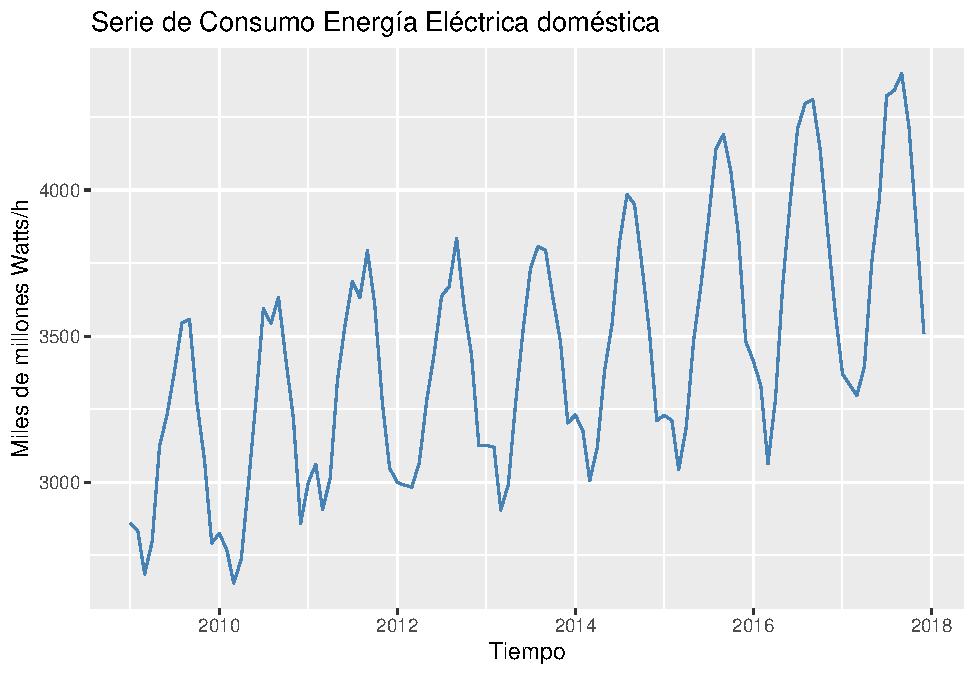
\includegraphics{TimeSeries_files/figure-latex/plotBaseSeries-1.pdf}
\caption{\label{fig:plotBaseSeries}Gráfica con ggplot usando programación nativa de R}
\end{figure}

La gráfica \ref{fig:plotBaseSeries} es adecuada ya que usa una potente herramienta de graficación como lo es \emph{ggplot}, sin embargo, tuvo que crearse 3 diferentes objectos, una base de datos llamada \emph{CONELDO.base}, un vector donde se encuentran los valores de la serie de tiempo \_CONELDO \_y un vector que recibe el nombre de \emph{time} el cual contiene una secuencia de fechas. Si se usará el objeto time series (ts) estas declaraciones no serían necesarias pues en este objeto se indexa el tiempo, así en el siguiente código puede observar que el resultado es equivalente al observado en la gráfica \ref{fig:plotBaseSeries}.

\begin{Shaded}
\begin{Highlighting}[]
\FunctionTok{plot}\NormalTok{(CONELDO.ts,  }\AttributeTok{xlab=} \StringTok{\textquotesingle{}Tiempo\textquotesingle{}}\NormalTok{, }\AttributeTok{ylab =} \StringTok{\textquotesingle{}Miles de millones Watts/h\textquotesingle{}}\NormalTok{,}
     \AttributeTok{main =} \StringTok{\textquotesingle{}Serie de Consumo Energía Eléctrica doméstica\textquotesingle{}}\NormalTok{,}
     \AttributeTok{col=}\StringTok{\textquotesingle{}steelblue\textquotesingle{}}\NormalTok{)}
\end{Highlighting}
\end{Shaded}

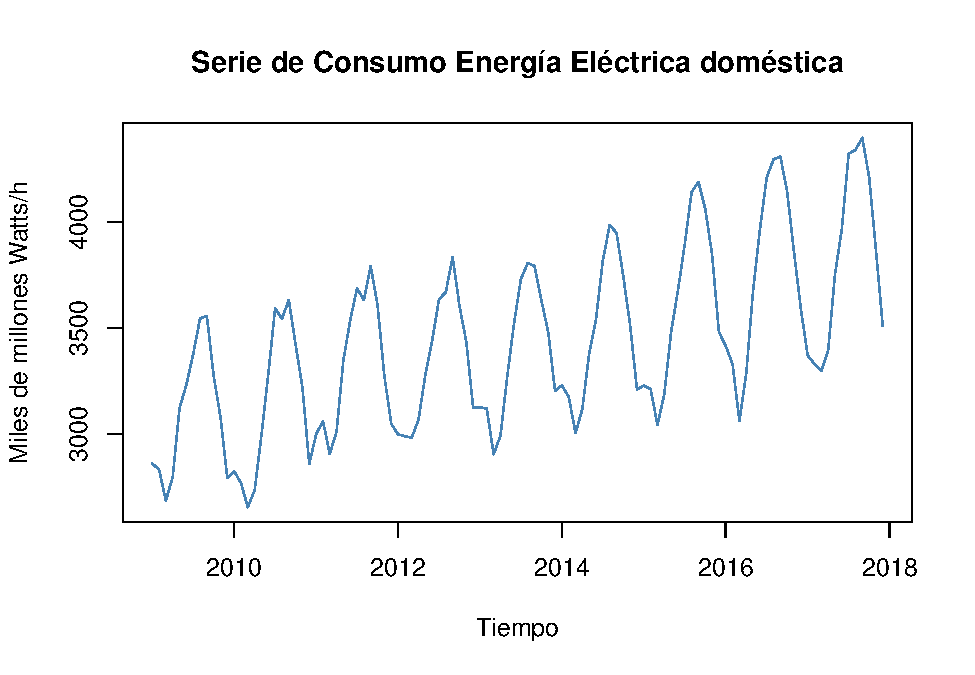
\includegraphics{TimeSeries_files/figure-latex/plotSerie-1.pdf}
Otra manera de poder graficar los datos a través de R es basándose en la librería \emph{xts}, este paquete incorpora una extensión al objeto \emph{ts} que viene por defecto en la instalación de R. El beneficio de \emph{xts} es que se pueden implementar varios tipos de gráficas auxiliares de series de tiempo, dentro del proceso de graficación ayuda a generar gráficas con un mayor control sobre los ejes además de añadir líneas en puntos de interés para ubicar mejor el tiempo y etiquetas más personalizadas. El proceso es similar al obtenido en la figura @ref\{fig:plotSerie\}, sin embargo , es necesario convertir el objeto \textbf{ts} a uno \textbf{xts}, para ello se usará la función \emph{as.xts()}, además sobre la gráfica se añadirá la opción \emph{major.ticks} para añadir etiquetas en el eje de las \(X\) según lo indiquemos, dentro de este parámetro se pueden indicar especificar los siguientes valores, `auto',`minute', `hours', `days', `weeks', `months', `quarters', y `years', pare periodos, automático, minutos, horas, días, semanas, meses, trimestres y años, respectivamente.

\begin{Shaded}
\begin{Highlighting}[]
\FunctionTok{library}\NormalTok{(xts)}
\NormalTok{CONELDO.xts }\OtherTok{=} \FunctionTok{as.xts}\NormalTok{(CONELDO.ts)}

\FunctionTok{plot}\NormalTok{(CONELDO.xts, }\AttributeTok{col =} \StringTok{\textquotesingle{}steelblue\textquotesingle{}}\NormalTok{, }
     \AttributeTok{grid.ticks.on =} \StringTok{\textquotesingle{}quarters\textquotesingle{}}\NormalTok{, }\CommentTok{\#Crea líneas verticales sobre la gráfica cada trimestre}
     \AttributeTok{major.ticks =} \StringTok{\textquotesingle{}quarters\textquotesingle{}}\NormalTok{,  }\CommentTok{\#Crea líneas verticales sobre la gráfica cada trimestre}
     \AttributeTok{minor.ticks =}\StringTok{\textquotesingle{}years\textquotesingle{}}\NormalTok{, }\CommentTok{\# Escribe la etiqueta de los meses cada cierto tiempo}
     \AttributeTok{grid.col =} \StringTok{\textquotesingle{}lightgrey\textquotesingle{}}\NormalTok{, }\CommentTok{\#color líneas verticales}
     \AttributeTok{main=}\StringTok{\textquotesingle{}Serie de Consumo Energía Eléctrica doméstica\textquotesingle{}}
     
\NormalTok{     )}
\end{Highlighting}
\end{Shaded}

\begin{figure}
\centering
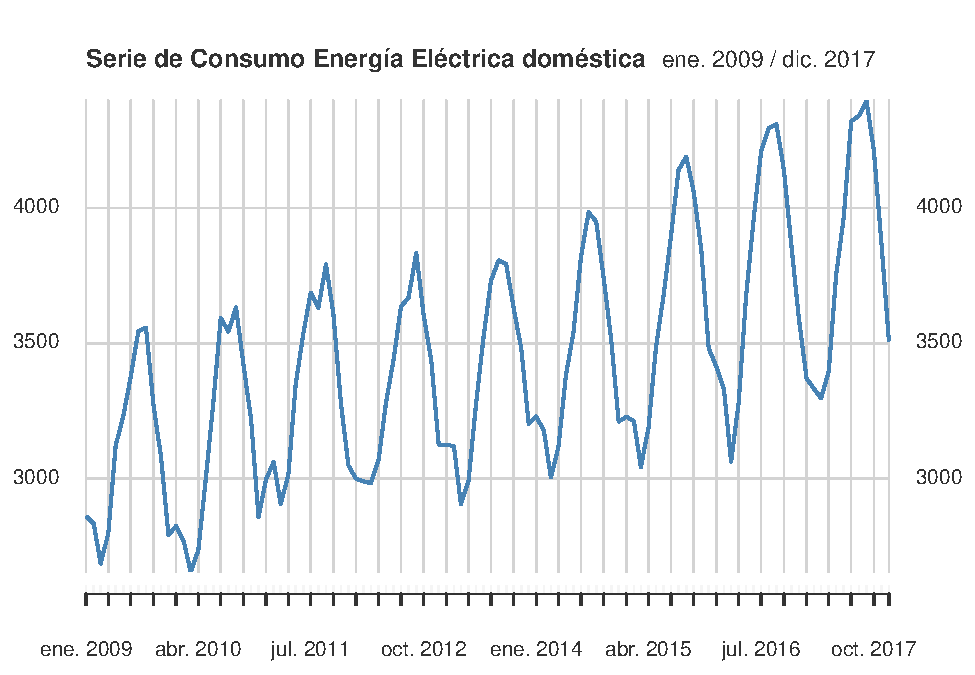
\includegraphics{TimeSeries_files/figure-latex/plotSeriexts-1.pdf}
\caption{\label{fig:plotSeriexts}Gráfica con plot usando el objeto xts}
\end{figure}

Las gráficas que se acaban de realizar son adecuadas, sin embargo, cada una de ellas tiene sus ventajas y desventajas, desde luego no son las únicas formas de graficar series de tiempo en R existen otros paquetes externos dentro de la cual destaca \emph{zoo}. A pesar de ello, a lo largo de este texto se usará de manera indiferente cada uno de los tres métodos mostrados anteriormente, ya que son los más generales y destacan en los siguiente:

\begin{itemize}
\tightlist
\item
  La gráfica con \emph{ggplot2} (figura \ref{fig:plotBaseSeries}) es la gráfica más estética de las 3 que se acaban de realizar, sin embargo, aunque es muy personalizable la cantidad de código que hay que considerar es mayor que los otros dos métodos presentados. Además por la manera en que se programa dicha gráfica no admitirá el objeto \emph{ts}, por lo que se tiene que crear una tabla o \emph{data.frame} en la cual en una columna deberá ser almacenado el valor de la serie de tiempo, y en otra las fechas o tiempos en que ocurrió cada observación.
\item
  La gráfica usando el objeto \emph{ts} y \emph{plot()} (figura \ref{fig:plotSerie}) es la gráfica más sencilla de implementar debido a que el comando \emph{plot()} acepta el objeto \emph{ts} y en dicha variable se encuentra indexado el tiempo, sólo será necesario indicar el nombre de las etiquetas y colores de la línea que sigue la serie de tiempo. El resultado es aceptable, sin embargo, estéticamente es la gráfica más sencilla de las presentadas anteriormente- Ya que no se tiene mucho control sobre las etiquetas del eje de las \(X\) y \(Y\) puede ocasionar que el lector se pierda en el tiempo y sea difícil comparar datos en un intervalo.
\item
  La gráfica usando el objeto \emph{xts} (figura \ref{fig:plotSeriexts}) es la más equilibrada de todas, el código es más sencillo y un poco menos vistosa que la gráfica \ref{fig:plotBaseSeries} usando \emph{ggplot} pero es más atractiva y ligeramente más elaborada que la gráfica \ref{fig:plotSerie}. Al incorporar y controlar las líneas verticales en el eje de las \(X\) permite que el lector se ubique mejor en el tiempo y pueda comprar resultados. El aspecto negativo es que se tendrá que crear un nuevo objeto del tipo \emph{xts} lo cual consumirá un pequeño pero existente lugar en la memoria y espacio de trabajo.
\end{itemize}

  \bibliography{book.bib,packages.bib}

\end{document}
